
\documentclass[border=1pt]{standalone}
\usepackage[T1]{fontenc}
\usepackage{newtxtext}
\usepackage{newtxmath}
\usepackage{amsmath}
\usepackage{tikz}
\usepackage{pgfplots}
\usepgfplotslibrary{groupplots}
\usetikzlibrary{arrows.meta}
\pgfplotsset{compat=1.18}

\definecolor{cclassical}{HTML}{2166ac}
\definecolor{clearned}{HTML}{b2182b}
\definecolor{cproposed}{HTML}{1a9850}
\definecolor{cref}{HTML}{7f7f7f}
\definecolor{clight}{HTML}{67a9cf}
\definecolor{cbandlo}{HTML}{f4a582}
\definecolor{cbandhi}{HTML}{92c5de}

% Figure text is sized for a 252 pt column: axis labels a touch under the
% 8 pt caption size, tick labels one step below that.
\newcommand{\figlab}{\fontsize{7.5}{8.5}\selectfont}
\newcommand{\figtick}{\fontsize{6.5}{7.5}\selectfont}
\newcommand{\fignote}{\fontsize{6}{7}\selectfont}

\pgfplotsset{
  every axis/.append style={
    line width=0.5pt,
    scale only axis,
    tick style={line width=0.4pt, black},
    tick pos=left,
    grid=major,
    grid style={gray!30, line width=0.3pt},
    label style={font=\figlab},
    tick label style={font=\figtick},
    title style={font=\figlab, yshift=-2pt},
    legend cell align=left,
    legend style={
      font=\fignote, draw=black!35, fill=white, fill opacity=0.92,
      text opacity=1, inner sep=1.2pt, row sep=-1.5pt, legend image post style={scale=0.7}},
  },
  every axis plot/.append style={line width=0.7pt, mark size=1.3pt},
}
\begin{document}
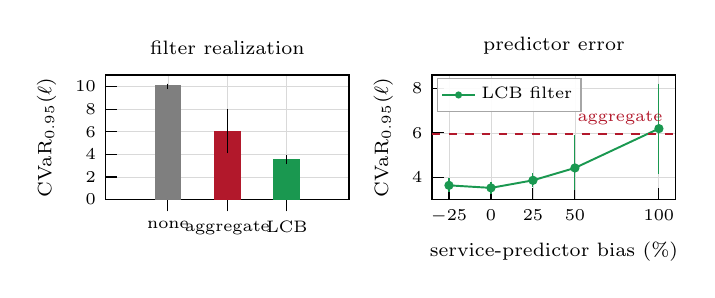
\begin{tikzpicture}
\begin{groupplot}[
  group style={group size=2 by 1, horizontal sep=30pt},
  width=88pt, height=45pt,
  ylabel={$\mathrm{CVaR}_{0.95}(\ell)$},
]
\nextgroupplot[title={filter realization}, ybar, bar width=9pt,
  xmin=-0.6, xmax=2.6, ymin=0, ymax=11,
  xtick={0,1,2}, xticklabels={none, aggregate, LCB},
  xticklabel style={font=\figtick}, ytick={0,2,4,6,8,10},
  enlarge x limits=0.14]
\addplot[fill=cref, draw=cref, bar shift=0pt, error bars/.cd, y dir=both, y explicit, error bar style={line width=0.4pt, black}, error mark options={line width=0.4pt, mark size=1pt, black}]
  table[x=x, y=y, y error plus=ep, y error minus=em] {
x y ep em
0 10 0 0
};
\addplot[fill=clearned, draw=clearned, bar shift=0pt, error bars/.cd, y dir=both, y explicit, error bar style={line width=0.4pt, black}, error mark options={line width=0.4pt, mark size=1pt, black}]
  table[x=x, y=y, y error plus=ep, y error minus=em] {
x y ep em
1 5.93966 1.78484 1.61495
};
\addplot[fill=cproposed, draw=cproposed, bar shift=0pt, error bars/.cd, y dir=both, y explicit, error bar style={line width=0.4pt, black}, error mark options={line width=0.4pt, mark size=1pt, black}]
  table[x=x, y=y, y error plus=ep, y error minus=em] {
x y ep em
2 3.52805 0.147835 0.146337
};
\nextgroupplot[title={predictor error}, xmin=-35, xmax=110,
  ymin=3.0, ymax=8.6, ytick={4,6,8}, xtick={-25,0,25,50,100},
  xlabel={service-predictor bias (\%)},
  legend style={at={(0.02,0.98)}, anchor=north west}]
\addplot[cproposed, mark=*, error bars/.cd, y dir=both, y explicit,
  error bar style={line width=0.4pt}, error mark options={line width=0.4pt, mark size=1pt}]
  table[x=x, y=y, y error plus=ep, y error minus=em] {
x y ep em
-25 3.64203 0.189707 0.168778
0 3.52805 0.147835 0.146337
25 3.86756 0.194885 0.195092
50 4.42464 1.36816 0.881745
100 6.19351 1.90281 1.91048
};

\addlegendentry{LCB filter}
\addplot[clearned, dashed, line width=0.6pt, forget plot] coordinates {(-35,5.93966) (110,5.93966)};
\node[font=\fignote, text=clearned, anchor=south east] at (axis cs:108,5.93966) {aggregate};
\end{groupplot}
\end{tikzpicture}
\end{document}
